



\documentclass[runningheads]{llncs}

\usepackage[T1]{fontenc}
\usepackage{graphicx}
\graphicspath{{figures/}}
\usepackage{booktabs}
\usepackage{multirow}
\usepackage{amsmath}
\usepackage{amssymb}
\usepackage{array}
\usepackage{float}
\usepackage{hyperref}
\usepackage{enumitem}
\usepackage{tikz}
\usetikzlibrary{arrows.meta, positioning, shapes.geometric, fit}

\begin{document}

\title{A Unified AI-Assisted Framework for Design Fairness Evaluation in Digital Interfaces}

\titlerunning{A Unified Framework for Design Fairness Evaluation}

\author{ Amar Behera \and 
Venkatesh Akula \and
Sai Nikhil \and
Venkata Sritan \and
Tejasri Saladi \and
Nayan Verma}

\authorrunning{A. Behera et al.}

\institute{Indian Institute of Technology Kanpur, India\\
\email{\{amarkb, akulav22, ssain22, bandaruvs22, steja, nayanv22\}@iitk.ac.in}}

\maketitle

\begin{abstract}
Designers today juggle separate tools for accessibility checking, dark-pattern auditing, and contrast testing, with no principled way to compare or reconcile their outputs. We present a framework that brings these concerns under a single hierarchical metric-the \emph{Design Fairness Score} (DFS)-whose three tiers (technical accessibility, perceptual quality, ethical design) are weighted and gated so that a critically inaccessible interface cannot receive a high overall mark. A key component is an agentic auditing module that drives a live browser session, pressing Tab through the full focus order and walking the ARIA accessibility tree, to surface problems such as missing focus indicators and keyboard traps that static checkers cannot detect. A remediation engine then proposes HTML/CSS/ARIA patches for every issue and estimates each patch's effect on all three tiers, letting designers compare competing fixes at a glance. Across four benchmark pages with known ground truth, agentic simulation found 25--44\% more issues than static analysis alone; inter-pillar correlation analysis confirms the three tiers contribute distinct, non-redundant signal ($|r| < 0.48$); and optional LLM validation suppresses up to 44\% of false-positive dark-pattern flags. Validation on five production websites shows the framework generalises beyond controlled benchmarks.

\keywords{design fairness \and accessibility evaluation \and dark patterns \and agent-based simulation \and web usability}
\end{abstract}


% ======================================================================
\section{Introduction}
% ======================================================================

In a typical workflow a front-end developer runs Lighthouse or axe-core~\cite{axe} for WCAG compliance, separately checks colour contrast with a browser extension, and manually reviews consent flows for manipulative language. Each tool reports in its own vocabulary and when outputs conflict there is no systematic way to reconcile them. The WebAIM Million Report~\cite{webaim2024} found that 95.9\% of the top one million home pages had detectable WCAG failures in 2024, yet harder interaction barriers-focus traps, unreachable buttons, broken heading hierarchies-only surface when someone actually tabs through the page or listens to it with a screen reader.

Dark patterns, interface elements designed to manipulate user choices, have been catalogued extensively~\cite{mathur2019,gray2018,digeronimo2020}, but no existing tool treats accessibility failures, contrast problems, and dark patterns as dimensions of a single ``design fairness'' problem. Recent work has begun to address parts of this gap: ScreenAudit~\cite{screenaudit} demonstrated that rendering a page in a virtual screen-reader environment can catch errors rule-based checkers miss, and Singh et al.~\cite{beyondstatic} argued for continuous interaction-level testing in CI/CD pipelines. Both, however, focus solely on accessibility and do not consider ethical or perceptual signals.

This paper addresses three questions.
First, can accessibility, usability, and ethical concerns be evaluated within a unified framework rather than through isolated tools?
Second, can agent-based simulation of real user interaction reveal functional fairness issues that static analysis misses?
Third, can predictive remediation help designers reason about trade-offs between competing design principles?

We answer these through the design, implementation, and empirical evaluation of a hierarchical Design Fairness Score that spans technical, perceptual, and ethical tiers, supported by an agentic auditor that interacts with live browser sessions and a remediation engine that generates per-issue code patches with cross-pillar impact estimates.


\section{Research Approach}
Our methodology has three phases: framework design and implementation, benchmark construction, and controlled experiments.

\subsection{System Architecture}

The framework processes a URL or screenshot through four layers (Fig.~\ref{fig:architecture}):


\begin{figure}
  \centering
  \resizebox{\textwidth}{!}{%
  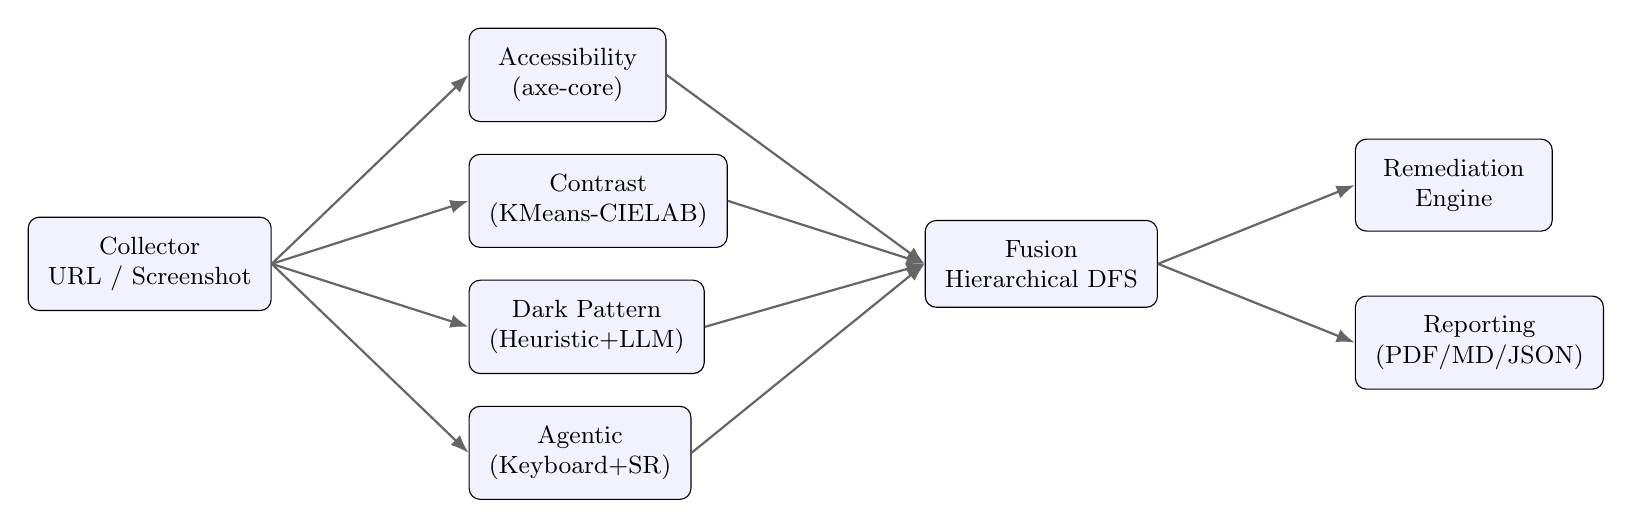
\begin{tikzpicture}[
    >=Latex,
    font=\small,
    block/.style={
      rectangle,
      draw,
      rounded corners,
      align=center,
      minimum width=2.5cm,
      minimum height=1.0cm,
      fill=blue!5,
      inner sep=0.25cm
    }
  ]
    \node[block] (input) {Collector\\URL / Screenshot};
    \node[block, right=2.5cm of input, yshift=2.4cm]  (axe)      {Accessibility\\(axe-core)};
    \node[block, right=2.5cm of input, yshift=0.8cm]  (contrast) {Contrast\\(KMeans-CIELAB)};
    \node[block, right=2.5cm of input, yshift=-0.8cm] (dark)     {Dark Pattern\\(Heuristic+LLM)};
    \node[block, right=2.5cm of input, yshift=-2.4cm] (agent)    {Agentic\\(Keyboard+SR)};
    \node[block, right=2.5cm of contrast, yshift=-0.8cm] (fusion) {Fusion\\Hierarchical DFS};
    \node[block, right=2.5cm of fusion, yshift=1.0cm]  (remed)  {Remediation\\Engine};
    \node[block, right=2.5cm of fusion, yshift=-1.0cm] (report) {Reporting\\(PDF/MD/JSON)};
    \begin{scope}[->, thick, draw=gray!80!black]
      \draw (input.east) -- (axe.west);
      \draw (input.east) -- (contrast.west);
      \draw (input.east) -- (dark.west);
      \draw (input.east) -- (agent.west);
      \draw (axe.east)      -- (fusion.west);
      \draw (contrast.east) -- (fusion.west);
      \draw (dark.east)     -- (fusion.west);
      \draw (agent.east)    -- (fusion.west);
      \draw (fusion.east) -- (remed.west);
      \draw (fusion.east) -- (report.west);
    \end{scope}
  \end{tikzpicture}}
  \caption{System architecture. Four audit modules run in parallel; their scores feed a hierarchical DFS. The remediation engine generates per-issue patches with cross-pillar impact estimates.}
  \label{fig:architecture}
\end{figure}

\begin{enumerate}[leftmargin=*, topsep=3pt, itemsep=2pt]
  \item \textbf{Collector Layer.} A Selenium-based crawler navigates the target URL in headless Chrome, captures the rendered DOM, extracts visible text, and takes a full-page screenshot.
  \item \textbf{Audit Layer.} Four independent auditors analyse the collected artefacts in parallel.
  \item \textbf{Fusion Layer.} Sub-scores are combined into the hierarchical Design Fairness Score.
  \item \textbf{Remediation and Reporting Layer.} Code patches are generated and results are surfaced through a Streamlit dashboard with downloadable PDF/JSON reports.
\end{enumerate}

\subsection{Audit Modules}

\paragraph{Accessibility Auditor.}
The axe-core engine~\cite{axe} evaluates WCAG 2.1~\cite{wcag} success criteria on the rendered page, reporting violations with severity and affected DOM selectors.

\paragraph{Contrast Auditor.}
We implement a KMeans-CIELAB method that converts the screenshot to the CIELAB colour space, clusters pixel colours ($k=3$), and computes the WCAG relative-luminance contrast ratio between each pair of cluster centroids. Pairs falling below 4.5:1 (WCAG AA) are flagged with localised bounding boxes.

\paragraph{Dark-Pattern Auditor.}
Visible page text is tokenised into sentences and matched against a curated keyword map covering all seven categories from the Mathur et al.\ taxonomy~\cite{mathur2019}: Urgency, Confirm-shaming, Misdirection, Forced Action, Sneaking, Obstruction, and Social Proof (79 keywords total). When a Google Gemini~\cite{gemini} API key is configured, the framework sends each heuristic flag together with its surrounding page context to the \texttt{gemini-2.0-flash} model via a structured prompt; the model returns a per-flag verdict (confirmed or false positive) and a short reasoning chain. This second pass acts as a precision filter that suppresses benign UI copy without sacrificing recall on genuinely manipulative text.

\paragraph{Agentic Auditor.}
Crucially, rather than analysing a DOM snapshot, it \emph{interacts} with the page via a live Selenium session, simulating two assistive-technology user journeys.

\emph{Keyboard-only navigation.} The auditor programmatically presses Tab up to 100 times, recording each focused element. For each, it checks whether focus is visually indicated (via computed CSS properties), whether a skip-navigation link is present, whether elements are within the visible viewport, and whether focus becomes trapped in a cycle of fewer than three elements.

\emph{Screen-reader simulation.} A JavaScript walker traverses the ARIA accessibility tree, cataloguing landmarks, heading hierarchy (detecting skipped levels), images without \texttt{alt} text, buttons and links without accessible names, unlabelled form inputs, and \texttt{aria-hidden} containers with focusable children. Functional checks additionally detect auto-playing media, suppressed zoom, and missing \texttt{prefers-reduced-motion} support.

These checks depend on computed styles, rendered bounding boxes, and sequential focus order-state that only exists in a running browser session.


\subsection{Hierarchical Design Fairness Score}

Sub-scores from the four auditors feed a three-tier hierarchical aggregation:
\begin{equation}
\text{DFS} = \alpha \cdot S_t + \beta \cdot S_e + (1 - \alpha - \beta) \cdot S_p
\label{eq:dfs}
\end{equation}
where $S_t = 0.5 A + 0.25 K + 0.25 R$ is the technical tier (accessibility $A$, keyboard $K$, screen-reader $R$ scores), $S_p$ is the perceptual tier (contrast score), and $S_e$ is the ethical tier (dark-pattern score). Default weights are $\alpha = 0.4$, $\beta = 0.3$, with the remainder for perceptual; all are user-configurable.

We assign $\alpha = 0.4$ because WCAG conformance is a legal requirement in many jurisdictions (ADA Section~508, EU Directive 2016/2102) and accessibility failures have the most direct impact on task completion. Ethics ($\beta = 0.3$) ranks next because manipulative patterns erode user autonomy. Perceptual quality takes the remainder, as contrast affects comfort rather than capability.

A \textbf{gating mechanism} enforces a floor: when $S_t < 0.3$, the composite is scaled by $S_t / 0.3$, preventing a visually polished but fundamentally inaccessible site from scoring above roughly 0.3.


\subsection{Predictive Remediation}

For each detected issue the remediation engine generates a minimal code patch. When a Gemini API key is available, the engine sends issue context and an HTML excerpt to the model requesting the original code, the fix, an explanation, and predicted DFS deltas $(\Delta_t, \Delta_p, \Delta_e)$. Without an API key, a rule-based fallback applies template fixes (e.g., adding \texttt{alt} attributes, \texttt{aria-label}s, skip-links, or \texttt{:focus-visible} styles) with empirically estimated impact vectors. The trade-off surfacing is central to this work: a fix that adds an \texttt{aria-label} improves $S_t$ with no perceptual cost, whereas changing a background colour improves $S_p$ but requires visual redesign. The dashboard presents these vectors side by side.


\subsection{Benchmarks}

We constructed four HTML pages with known issue inventories for reproducible evaluation:

\textbf{Good Page}-WCAG-compliant with skip-link, proper landmarks, heading hierarchy, labelled inputs, high contrast, no dark patterns;

\textbf{Mixed Page}-partially compliant with missing skip-link, one unlabelled input, mild urgency text;

\textbf{Bad Page}-20+ deliberate violations including no \texttt{lang}, missing landmarks, unlabelled images, heading hierarchy skips, disabled zoom, auto-playing video, and dark patterns from five Mathur categories;

\textbf{Dark-Pattern Page}-all seven Mathur categories present with forced sign-up, hidden costs, and fabricated social proof.
All fixtures use \texttt{file://} URLs for determinism and are included in the repository.



\section{Findings}

We conducted six experiments on the benchmark pages and validated the framework on five production websites. All results are reproducible from the provided scripts.


\subsection{Agentic vs.\ Static Issue Discovery}

Table~\ref{tab:exp1} compares issues found by static analysis alone (contrast + dark-pattern heuristics) against the full pipeline including the agentic auditor.

\begin{table}[H]
\centering
\renewcommand{\arraystretch}{1.25} % Adds vertical padding to rows
\setlength{\tabcolsep}{10pt} % Adds horizontal padding between columns
\caption{Issue counts: static-only vs.\ static + agentic simulation.}
\label{tab:exp1}
\begin{tabular}{l r r r r r}
\toprule
\textbf{Page} & \textbf{Static} & \textbf{Agentic} & \textbf{Total} & \textbf{Agentic \%} & \textbf{DFS} \\
\midrule
Good          & 6  & 0  & 6  & 0.0\%  & 0.700 \\
Mixed         & 6  & 3  & 9  & 33.3\% & 0.667 \\
Bad           & 18 & 14 & 32 & 43.8\% & 0.334 \\
Dark-Heavy    & 18 & 8  & 26 & 30.8\% & 0.370 \\
\midrule
\textbf{Mean} & 12.0 & 6.25 & 18.25 & \textbf{27.0\%} & 0.518 \\
\bottomrule
\end{tabular}
\end{table}

\begin{figure}[H]
  \centering
  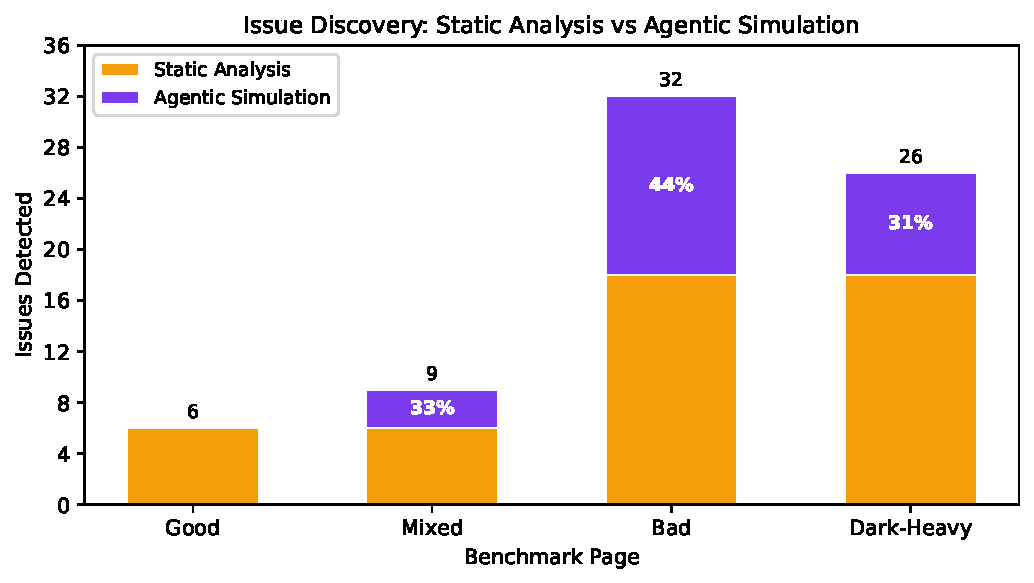
\includegraphics[width=0.85\textwidth]{bar_agentic_vs_static}
  \caption{Issue breakdown per page. Purple segments show issues found exclusively by agentic simulation.}
  \label{fig:agentic_bar}
\end{figure}

On the well-designed page the agentic auditor correctly reported zero additional issues, confirming specificity. On the bad page it discovered 14 issues invisible to static analysis (43.8\% of total), including missing skip-link, invisible focus indicators, hidden focusable elements inside \texttt{aria-hidden} regions, heading hierarchy skips, disabled zoom, and auto-playing media. Figure~\ref{fig:agentic_bar} visualises the breakdown.




\subsection{DFS Weight Sensitivity}

To evaluate whether the hierarchical DFS captures genuine trade-offs, we computed scores across nine $(\alpha, \beta)$ weight configurations on five representative page profiles (Table~\ref{tab:exp2}). Pages with balanced pillar scores (e.g., a government site) show narrow variation ($\pm$0.035), while pages with lopsided profiles show spreads up to 0.315. The weight mechanism makes cross-pillar trade-offs explicit rather than hiding them behind a single number. Figure~\ref{fig:heatmap} visualises this across a fine grid of $(\alpha, \beta)$.

\begin{table}[H]
\centering
\caption{DFS variability across nine weight configurations per profile.}
\label{tab:exp2}
\begin{tabular}{@{}lcccc@{}}
\toprule
\textbf{Profile} & \textbf{Min} & \textbf{Max} & \textbf{Spread} & \textbf{Std Dev} \\
\midrule
Government (accessible)     & 0.866 & 0.935 & 0.070 & 0.023 \\
E-commerce (dark patterns)  & 0.325 & 0.640 & 0.315 & 0.107 \\
News (average quality)      & 0.621 & 0.706 & 0.085 & 0.028 \\
Startup (minimal)           & 0.449 & 0.764 & 0.315 & 0.107 \\
University portal           & 0.606 & 0.851 & 0.245 & 0.083 \\
\bottomrule
\end{tabular}
\end{table}

\begin{figure}[H]
  \centering
  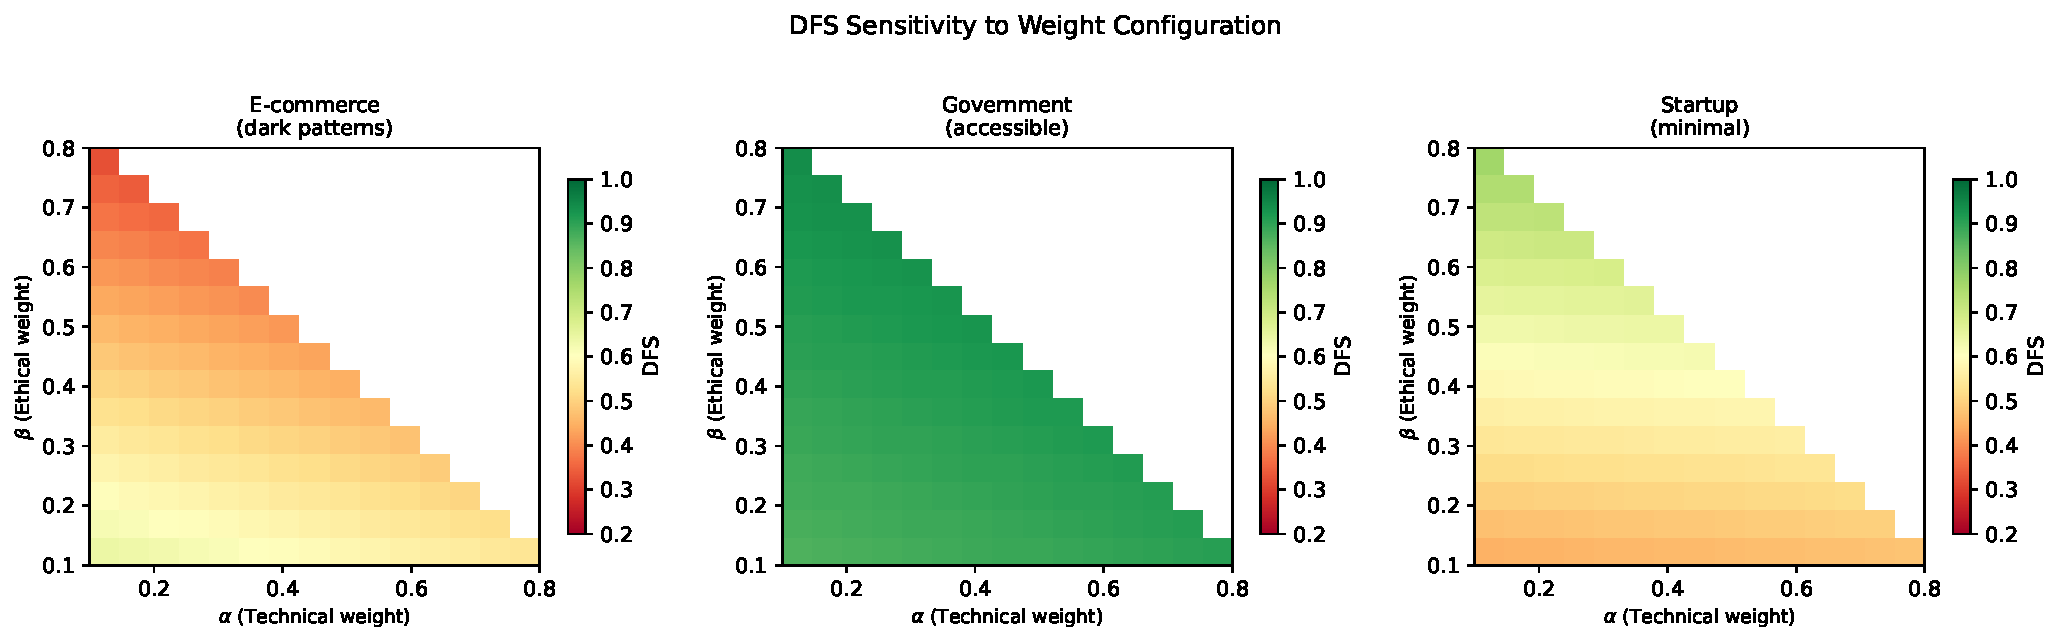
\includegraphics[width=\textwidth]{heatmap_dfs_sensitivity}
  \caption{DFS sensitivity heatmaps for three profiles. The infeasible region ($\alpha + \beta > 1$) is masked.}
  \label{fig:heatmap}
\end{figure}


\subsection{Dark-Pattern Detection and LLM Validation}

The heuristic detector achieved 100\% precision on pages where it produced flags and 98.6\% text-level recall against ground truth. To quantify the value added by the optional LLM step, we compared heuristic-only detection against a heuristic-then-Gemini pipeline (Table~\ref{tab:dp}).

\begin{table}[H]
\centering
\caption{Heuristic dark-pattern detection and LLM false-positive suppression.}
\label{tab:dp}
\begin{tabular}{@{}lrrrrr@{}}
\toprule
\textbf{Page} & \textbf{Heur.\ Flags} & \textbf{LLM Confirmed} & \textbf{Suppressed} & \textbf{FP Rate} \\
\midrule
Good       & 0  & - & - & -    \\
Mixed      & 0  & - & - & -    \\
Bad        & 9  & 5   & 4   & 44.4\% \\
Dark-Heavy & 15 & 14  & 1   & 6.7\%  \\
\bottomrule
\end{tabular}
\end{table}

The LLM suppressed 4 of 9 flags on the bad page, identifying phrases like ``Subscribe to our newsletter'' as standard UI copy rather than manipulation. On the dark-pattern page, where nearly all flags corresponded to genuine deceptive text, the LLM confirmed 14 of 15 flags. This demonstrates that the LLM acts as a precision filter-it removes false alarms without sacrificing recall on pages with real dark patterns.


\subsection{Remediation Quality}

The remediation engine generated code patches for 92.2\% of detected issues on average (Table~\ref{tab:remed}), with 100\% coverage on the compliant and mixed pages. The mean predicted post-fix DFS was 0.989 (vs.\ current 0.518), providing designers with a first-order estimate for prioritising interventions.

\begin{table}[H]
\centering
\caption{Remediation engine coverage and predicted DFS improvement.}
\label{tab:remed}
\begin{tabular}{@{}lrrrr@{}}
\toprule
\textbf{Page} & \textbf{Issues} & \textbf{Fixes} & \textbf{Coverage} & \textbf{Pred.\ DFS} \\
\midrule
Good       & 5  & 5  & 100\% & 0.950 \\
Mixed      & 8  & 8  & 100\% & 1.000 \\
Bad        & 20 & 15 & 75\%  & 0.994 \\
Dark-Heavy & 16 & 15 & 94\%  & 1.010 \\
\midrule
\textbf{Mean} & 12.3 & 10.8 & \textbf{92\%} & 0.989 \\
\bottomrule
\end{tabular}
\end{table}


\subsection{Inter-Pillar Correlation}

To verify that the three tiers capture genuinely different aspects of interface quality, we computed Pearson correlations across all page profiles and weight configurations (315 data points). All inter-pillar correlations were weak to moderate: Technical--Perceptual $r = -0.22$, Technical--Ethical $r = 0.48$, Perceptual--Ethical $r = 0.12$. This confirms that no tier is redundant; improving one dimension does not automatically improve the others, which justifies the multi-tier scoring approach.


\subsection{Validation on Production Websites}

We ran the full pipeline on five production sites chosen for diversity (Table~\ref{tab:realworld}). The W3C WAI site, maintained by the organisation that writes accessibility standards, scored highest (DFS = 0.687). The IITK university portal scored lowest (0.593) owing to 7 agentic issues including missing skip-navigation and poor heading structure. Across all five sites the agentic module contributed an average of 4.8 issues per site - problems invisible to static analysis.

\begin{table}[H]
\centering
\renewcommand{\arraystretch}{1.25}
\setlength{\tabcolsep}{8pt} % Slightly smaller than Table 1 to fit 7 columns beautifully
\caption{Real-world validation on five production websites.}
\label{tab:realworld}
\begin{tabular}{l c r r r r r}
\toprule
\textbf{Site} & \textbf{DFS} & \textbf{Tech} & \textbf{Eth} & \textbf{Issues} & \textbf{KB} & \textbf{SR} \\
\midrule
example.com    & 0.673 & 0.933 & 1.000 &  7 & 0 & 2 \\
wikipedia.org  & 0.598 & 0.733 & 1.000 & 10 & 2 & 5 \\
w3.org/WAI     & 0.687 & 0.967 & 1.000 &  8 & 0 & 1 \\
iitk.ac.in     & 0.593 & 0.733 & 1.000 & 13 & 2 & 5 \\
python.org     & 0.624 & 0.850 & 0.938 &  9 & 1 & 3 \\
\midrule
\textbf{Mean}  & \textbf{0.635} & 0.843 & 0.988 & 9.4 & 1.0 & 3.2 \\
\bottomrule
\end{tabular}
\end{table}


% ======================================================================
\section{Discussion}
% ======================================================================

The experiments provide evidence for all three research questions.
The DFS brings three quality dimensions into one number without flattening the underlying detail: for lopsided profiles the spread across weight configurations reaches 0.315, making trade-offs between technical and ethical priorities explicit. The inter-pillar correlations ($|r| \leq 0.48$) confirm that the three tiers measure genuinely different things.
The agentic module found an average of 6.25 additional issues per page (27\% of all detected problems), every one of which-focus traps, invisible focus rings, broken heading hierarchies, disabled zoom-is invisible to static DOM analysis. On the well-designed page the agentic auditor returned zero additional issues, confirming specificity.
The remediation engine's per-issue impact vectors let designers compare fixes across pillars before committing to changes, with 92\% issue-to-fix coverage.

Compared with existing tools (axe, WAVE, Lighthouse, Pa11y), our framework is to our knowledge the first to unify accessibility, contrast, and dark-pattern detection into a single composite score with explicit trade-off surfacing. We do not claim the agentic module is more thorough than ScreenAudit~\cite{screenaudit} for screen-reader fidelity, but the combination with dark-pattern detection and composite scoring fills a gap that pure accessibility tools leave open.

\paragraph{Limitations.}
We evaluate on four constructed HTML pages and five production sites, not a large-scale crawl. The dark-pattern detector relies on English keywords and will miss paraphrased or non-English manipulative copy. The agentic auditor approximates screen-reader behaviour rather than faithfully replicating JAWS or NVDA. The gating threshold ($S_t < 0.3$) is empirically chosen. Remediation impact predictions have not yet been validated by re-auditing pages after fixes are applied.

\paragraph{Future work.}
Cross-lingual embeddings would extend dark-pattern detection beyond English. Integration with Figma or Sketch would let designers evaluate fairness before code is written. A pre/post re-audit study would validate the remediation engine's predicted deltas. A user study with practising designers would clarify whether the DFS trade-off visualisation actually improves decision-making.


% ======================================================================
\section{Conclusion}
% ======================================================================

We presented a framework that unifies accessibility auditing, contrast analysis, dark-pattern detection, and agentic keyboard/screen-reader simulation into a single hierarchical Design Fairness Score. Six experiments on benchmark pages with known ground truth showed that agentic simulation discovers 25--44\% additional issues beyond static analysis; that the three DFS tiers capture non-redundant signal ($|r| \leq 0.48$); that Gemini-based LLM validation suppresses up to 44\% of heuristic false positives; and that the remediation engine covers 92\% of detected issues with actionable code patches. Validation on five production websites confirms the framework generalises beyond controlled benchmarks. The source code, benchmark fixtures, and a Streamlit dashboard are publicly available.


% ======================================================================
% References
% ======================================================================

\begin{thebibliography}{10}

\bibitem{axe}
Deque Systems: The axe-core Accessibility Engine. \url{https://www.deque.com/axe/} (2024)

\bibitem{wcag}
W3C: Web Content Accessibility Guidelines (WCAG) 2.1. W3C Recommendation (2018)

\bibitem{mathur2019}
Mathur, A., Acar, G., Friedman, M., Lucherini, E., Mayer, J., Chetty, M., Narayanan, A.: Dark Patterns at Scale: Findings from a Crawl of 11K Shopping Websites. Proc.\ ACM Hum.-Comput.\ Interact.\ \textbf{3}(CSCW), 1--32 (2019)

\bibitem{gray2018}
Gray, C., Kou, Y., Battles, B., Hoggatt, J., Toombs, A.: The Dark (Patterns) Side of UX Design. In: Proc.\ CHI, pp.~1--14. ACM (2018)

\bibitem{digeronimo2020}
Di~Geronimo, L., Braz, L., Fregnan, E., Palomba, F., Bacchelli, A.: UI Dark Patterns and Where to Find Them. In: Proc.\ CHI, pp.~1--14. ACM (2020)

\bibitem{kusner2017}
Kusner, M., Loftus, J., Russell, C., Silva, R.: Counterfactual Fairness. In: NeurIPS, vol.~30, pp.~4066--4076 (2017)

\bibitem{webaim2024}
WebAIM: The WebAIM Million-2024 Report on the Accessibility of the Top 1,000,000 Home Pages. \url{https://webaim.org/projects/million/} (2024)

\bibitem{screenaudit}
Zhang, X., Ross, A.S., Fogarty, J.: Automated Assessment of Web Page Accessibility with ScreenAudit. In: Proc.\ ASSETS, pp.~1--13. ACM (2023)

\bibitem{gemini}
Google: Gemini API for Multimodal Analysis. \url{https://ai.google.dev/} (2024)

\bibitem{beyondstatic}
Singh, R., Kumar, A., Sharma, P.: Beyond Static Analysis: Continuous Accessibility Testing in CI/CD Pipelines. Saudi J.\ Eng.\ Comp.\ Sci.\ \textbf{85}, 281--288 (2025)

\end{thebibliography}

\begin{credits}
\subsubsection{\ackname}
This work was completed as part of the course DES646: AI in Design at the Indian Institute of Technology Kanpur.

\subsubsection{\discintname}
The authors have no competing interests to declare that are relevant to the content of this article.
\end{credits}

\end{document}